\documentclass[12pt]{article}
\usepackage[margin=1in]{geometry}

\usepackage{latexsym, amssymb, amsmath, amsfonts, amscd, amsthm}
\usepackage{enumerate, hyperref, multicol, tikz}

\theoremstyle{definition}
\newtheorem{definition}{Definition}[section]
\newtheorem{example}{Example}
\newtheorem{exercise}{Exercise}
\newtheorem{question}{Question}
\newtheorem*{notation*}{Notation}

\theoremstyle{theorem}
\newtheorem{fact}{Fact}
\newtheorem{lemma}{Lemma}
\newtheorem{proposition}{Proposition}
\newtheorem{theorem}{Theorem}
\newtheorem{corollary}{Corollary}

\newcommand{\NN}{\mathbb{N}}
\newcommand{\ZZ}{\mathbb{Z}}
\newcommand{\QQ}{\mathbb{Q}}
\newcommand{\RR}{\mathbb{R}}
\newcommand{\CC}{\mathbb{C}}
\newcommand{\FF}{\mathbb{F}}


\begin{document}
Google Scholar makes it easy to cite and manage sources using Bibtex by following these steps:
\begin{center}
	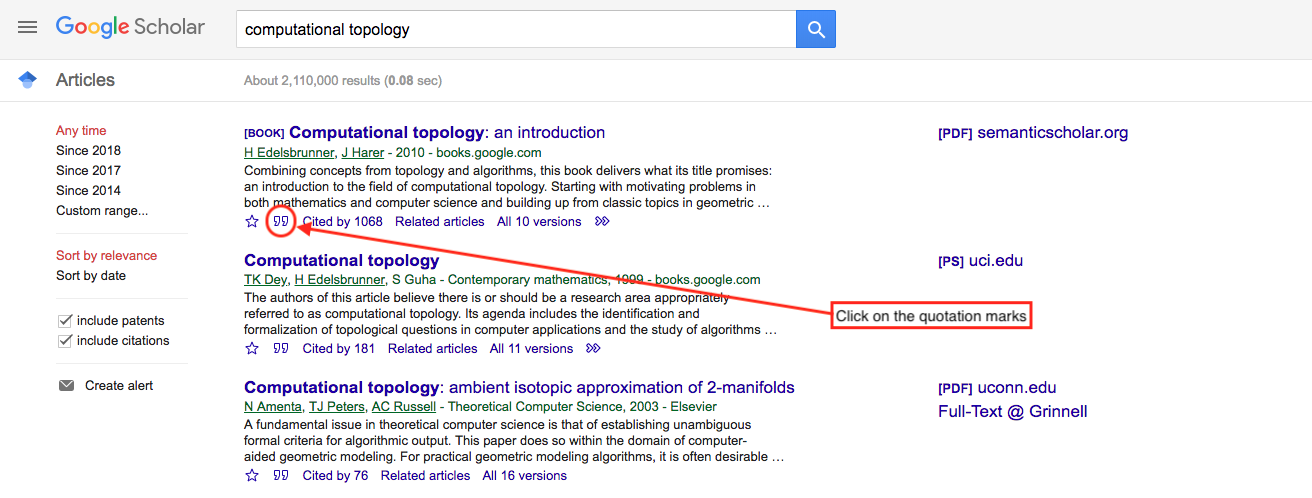
\includegraphics[width=1\linewidth]{step1}\\
	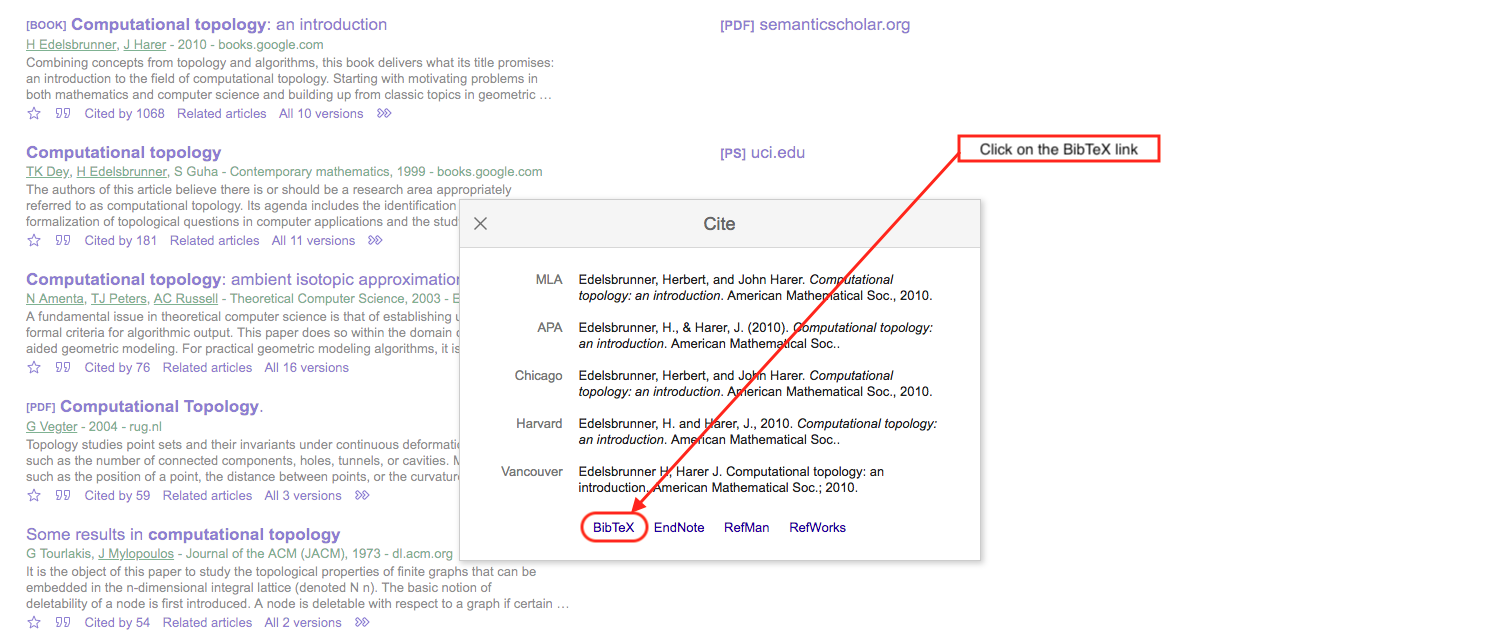
\includegraphics[width=1\linewidth]{step2}\\
	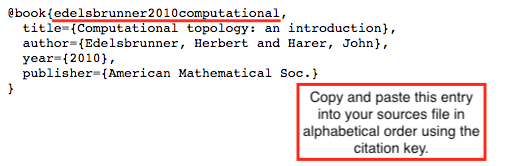
\includegraphics[width=.5\linewidth]{step3}\\
\end{center}

Other sites have similar features, if you dig a little.

Make sure the \verb|.bib| file you are using is in the same directory as your \verb|.tex| file. To make reference to an item in the bibliography, use the \verb|\cite{CITATION_KEY}| command. For example, we look to Edelsbrunner and Harer \cite{edelsbrunner2010computational} for our initial definitions and examples.

\bibliographystyle{plain}
\bibliography{sources}

\end{document}